\section{Introduction}
\label{sec:intro}
Animal languages have captured the curiosity of scientists for years and it has been proved that animals possess languages in their communications with others. Despite multiple attempts from different aspects, deciphering the complex intricate semantic meanings in animal communication systems remains a challenge ~\cite{andreas2022towards,scott2023animal}. Gaining a deeper understanding of animal language holds 
significant implications for unraveling their social structures, 
intelligence, and facilitating human-animal interactions. 

Among the vast array of animal languages, dog's language is
a good subject to study as they are one of the most popular pet animals and constantly interact with human beings via their vocal expressions.
Given the massive interactions between dogs and people during the domestication process, dogs' vocal behavior undergoes considerable changes ~\cite{jieyiacl2023, feddersen2000vocalization} and it is reasonable to infer that the diverse sounds emitted by dogs in varying scenes carry distinct significances.
Previous works on dog language have largely relied on experimental knowledge and heuristic
subjective observations, which depend on long-term experiences and costly 
data-collection and can be limited and prone to biases ~\cite{yin2002new,pongracz2010barking,farago2017dog}. Only coarse-grained meanings can be drawn given limited data and corresponding scenes from these studies. 
Our data-driven exploration is able to uncover fine-grained semantics with more context.
%\MY{Only coarse-grained meanings can be drawn given limited data and corresponding scenes from these studies.}
\begin{figure*}[t]
	\centering
	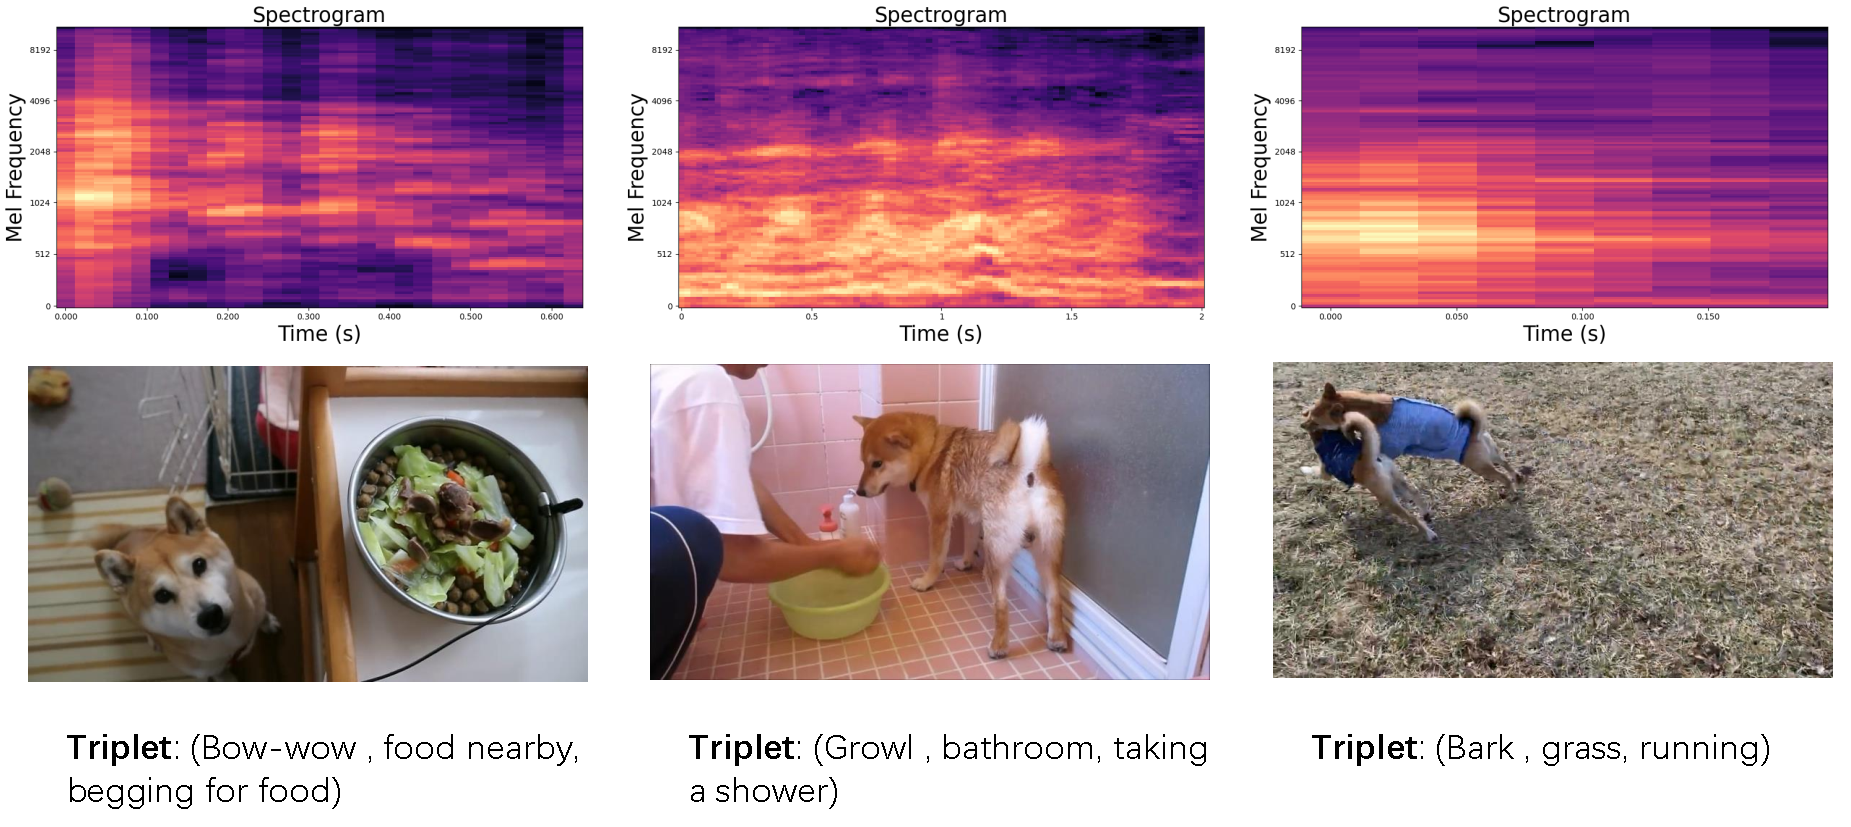
\includegraphics[width=0.95\textwidth]{images/intro.png}
	\caption{Introducing scenario: Spectrograms of dog sounds in the corresponding context. When the dog is begging for food, taking a shower, or running for a fight, its vocal spectrograms differ a lot. We mapped possible words extracted from dog barking audio with location and activity, forming our triplet dataset \texttt{<word, location, activity>}.
		\href{https://anonymous.4open.science/r/emnlp2023-937942/audios_in_paper/fig11.wav}{[Listen 1]}
		\href{https://anonymous.4open.science/r/emnlp2023-937942/audios_in_paper/fig12.wav}{[Listen 2]}
		\href{https://anonymous.4open.science/r/emnlp2023-937942/audios_in_paper/fig13.wav}{[Listen 3]}
	} %\MY{you need subfigure titles, e.g. ``Bow-wow''  under spectrogram, ``Food nearby, laying down'' under 1st picture}}
	%\KZ{Pls leave some spaces between the 3 pics on the bottom.}
	%to anywhere in the text! Every fig and table that you include in the paper must
	%be referred to somewhere!}}
	\label{fig:intropic}
\end{figure*}

For a wide range of vocalizations ~\cite{yeon2007vocal} dogs can produce when engaging with the external environment, the emotion of the dog, the surrounding environment the dog is located in, the activity the dog is doing, the object the dog interacts with, and even the age and gender of the dog may play a key factor in the sound the dog produces ~\cite{pongracz2005human,molnar2009dogs}.
Since Shiba Inu is a widely adopted dog at home and plenty of video data is available on YouTube, we choose this specific species to do our research. Hereby, we investigate the semantic meaning of the Shiba Inu dog sound according to two important factors of the context,  the \textit{location} and the \textit{activity} of the dog. 

 %\KZ{Give cites here.} 
 
%\JY{here add our advantages over previous work}



To understand the semantic meaning of dog language, there are several challenges: how to extract the meaningful word from audio clips and to ascertain if they show consistent patterns with context. 
In this work, we implement the first data-driven, evidence-based research 
sourced from social media to give fine-grained semantics for understanding 
the vocal language of Shiba Inu.
% In comparison, we propose a web-data-driven method that takes advantage of the large Internet resources, which saves collection costs as well as enlarges our data size. 
In inferring the context of the words, we construct triplets consisting of \texttt{<word, location, activity>}. We first explore the prior probability of each item in triplet to have a basic understanding of our data distribution. Then we investigate the possible pattern which could reveal the semantic meaning of dog word types. 

With this large quantity of data and our carefully-designed procedure for mapping words with context, we can take a closer look into the behaviors of animals and some hidden semantic patterns. For example, one kind of dog sound, bow-wow, is usually mixed with bark by previous researchers. However, in our work, we find that it shows the curiosity of dogs for the surroundings while bark doesn't have such meaning. Another example is related to ``growl'', traditionally seen as a low, guttural vocalization produced by animals as a warning, a sign of aggression, or to express anger\footnote{https://en.wikipedia.org/wiki/Growling}, while our analysis shows that ``growl'' for dogs may also be seen as a signal of positively interacting with humans. 
On the other hand, our method has more detailed contexts for analyzing animal languages, which will benefit future works. We identified as many as 11 locations and 12 activities, in which dogs might produce different vocal sounds to signify various meanings. 
%\KZ{You were already talking about gowling in the first para,now setting the stage for dog language seems too late.}
 
%\KZ{A bit too verbose here for giving the reason why we study dog language.
%I think the first two paras can be shortened and combined into one.}
%\MY{ In the 1st paragraph, you should focus on saying that why problem is important and why it is difficult to solve given previous effors. }
%\KZ{You need to cite more papers in the intro. At least cite two of Jieyi's
%papers?}


%\KZ{Why previous approach doesn't work well. E.g., bark and bow-wow are
%complicated and have not been given clear semantics.} explain above!!!

%Dog sounds can be classified into different types. The classification of these sounds is a interesting task, as it provides a framework for understanding the diverse vocal manifestations of dogs. We adopt the classification defined in Audioset, where dog sounds can be categorized into bark, yip, howl, bow-wow, growling, and whimper. Each of these categories present distinct vocal patterns of dogs, each carrying unique semantic connotations. Dogs will make different sound in different context. Here, we consider context to be determined by the actions of the dog at that time and the scene in which it is located. 
%\MY{You are correct that we need to say that verbal communications are to interact with outside world, hence we define the context i.e. their locations, and activity to analyse these interactions with certain words. Better give a few references that preliminary investigations indicate that dogs' sound are different given these conditions. }

 %\MY{This and the later para can be merged together, you don't want to go deep into too many details here to distract your readers}
%i.e., using same words under same context, we would determine that 
%these words are used to express certain meanings.  
%\KZ{The following two paras can be more concise.}



%\MY{This para is still verbose and detailed, you summarize your main idea in tackling the problem, and illustrate it here.}

 %to infer the context of the words we have extracted and to match the words and the context, 
%To tackle the challenges in aligning words with context, we process the audio to find words and remove the noisy parts then we classify these words into different types. Then, according to the corresponding words' timestamp, we go back to videos to find the activity and location (as shown in ~\figref{fig:intropic}).
%The classification of the words provides us with a framework for understanding the diverse vocal manifestations of dogs. 
%We adopt the definition of Audioset ~\cite{gemmeke2017audio}, where dog words can be categorized into the bark, yip, howl, bow-wow, growling, and whimper. 
%We analyze them in accordance with the corresponding context where a specific sound is produced. 

%For example, howl is used when there is food nearby, so it may implicate the desire for food. 
%We also explore sequences of words to find bi-gram semantic meaning. Some of our results support previous findings. For example, ``whimper'' can express attention seeking. We also yield new possible discoveries. For example, ``howl'' can be used as a signal for food. We aim to deepen our understanding of the complex communication system employed by dogs and eventually decipher their language by exploring the possible dog word meaning.
%\MY{Some of our results support previous findings that xxxx. We also yield new possible discoveries that xxx}

%Each of these categories present distinct vocal patterns and possible different meanings. Bark is the principal communication sound produced by dogs; Yip is a sharp high-pitched bark or cry, typically from a miniature dog; Howl is the long plaintive cry of a dog; Bow-wow is more tonal and less abrupt than a classic bark; Growling is a low, guttural vocalization; and whimper is a muted dog vocaliazation indicating submission, fear or pain.




%\JY{add their definitions and meanings here}
%For example, when the dog is running for fight, it will bark loudly with high frequency. Whereas begging for food, it will whimper with a soft and low voice. 

%\begin{table}[th]
%	\small
%	\begin{tabular}{p{0.15\columnwidth}|p{0.35\columnwidth}|p{0.35\columnwidth}}
%		\toprule
%		\textbf{Word} & \textbf{Definition} & \textbf{Meaning}\\ \midrule
%		Bark & ?
%		\\ \midrule
%		Yip & 
%		\\ \midrule
%		Howl &
%		\\\midrule
%		Bow-wow & 
%		\\\midrule
%		Growling & 
%		\\\midrule
%		Whimper & 
%		\\
%		\bottomrule
%	\end{tabular}
%	\caption{Overall findings of the analysis.}
%	\label{tab:worddefinition}
%\end{table}


%\MY{See? this para is somewhat lost, as previously it seems you have talked about how you aligned them and drew the conclusions, and now you start again talking about the triplets}
%\MY{This detailed explaination to our work can come later in the intro. Here you would say that the challenging part in understanding animal vocalization is to segment and extract meaningful words. By matching these distinct types of words to context, we can provide initial discoveries to animal semantics, that if they show consistent patterns, i.e. using same words under same context, we would determine that these words are used to express certain meanings}

Our main contributions are:
\begin{itemize}
	\item We propose a universal pipeline to process and analyze
dog-related videos on YouTube, so as to understand the lexical semantics of 
dog language. The framework is reusable to other animal species for which videos are available.
\item We are the first to implement data-driven research to study dog semantic language from webly data. We build a dataset \footnote{Code and dataset can be seen at \url{https://anonymous.4open.science/r/emnlp2023-937942/README.md}} that is the largest and contains 6 distinct words and corresponding context for exploring dog language. 
\item Through our investigation of dog sound patterns, we have uncovered several conclusions that align with existing human knowledge and previous research. Additionally, we have gained unique insights that are currently undefined.
\end{itemize}

%\cite{Gusfield:97}
